%!TEX root = ../report.tex

% 
% Related work
% 

\section{Related Work (~17pgs)}
\label{sec:rw}

There are several tools offered by the current \ac{ide}s. We focus on the development tools which help programmers to write code, one can also highlight other aspects, such as the supported \ac{pl}s.

The remaining of this section is organized as follows. Section~\ref{sec:gdide} describes the general design of \ac{ide}s. Section~\ref{sec:ide} briefly describes the actual commercial \ac{ide}s and its features. Section~\ref{sec:liveness} highlights the main tools used in live programming \ac{ide}s. Finally, Section~\ref{sec:gd} introduces the \ac{gd} area and its \ac{ide}s.

\subsection{General design of IDEs}
\label{sec:gdide}

The programming environment started as a \ac{case}. The main concern, of this technology is support all, or at least, substantial part of software process. So, the first \ac{case} system came up with a set of software tools, such as compilers, editors and debuggers put together on a host machine which was dedicated to program development~\cite{ivie1977programmer}. In order to understand how the tools work together and, eventually, howcan we add new tools in a existing \ac{ide}, let look more deeply at this system. 

\begin{figure}[h]
  \centering
  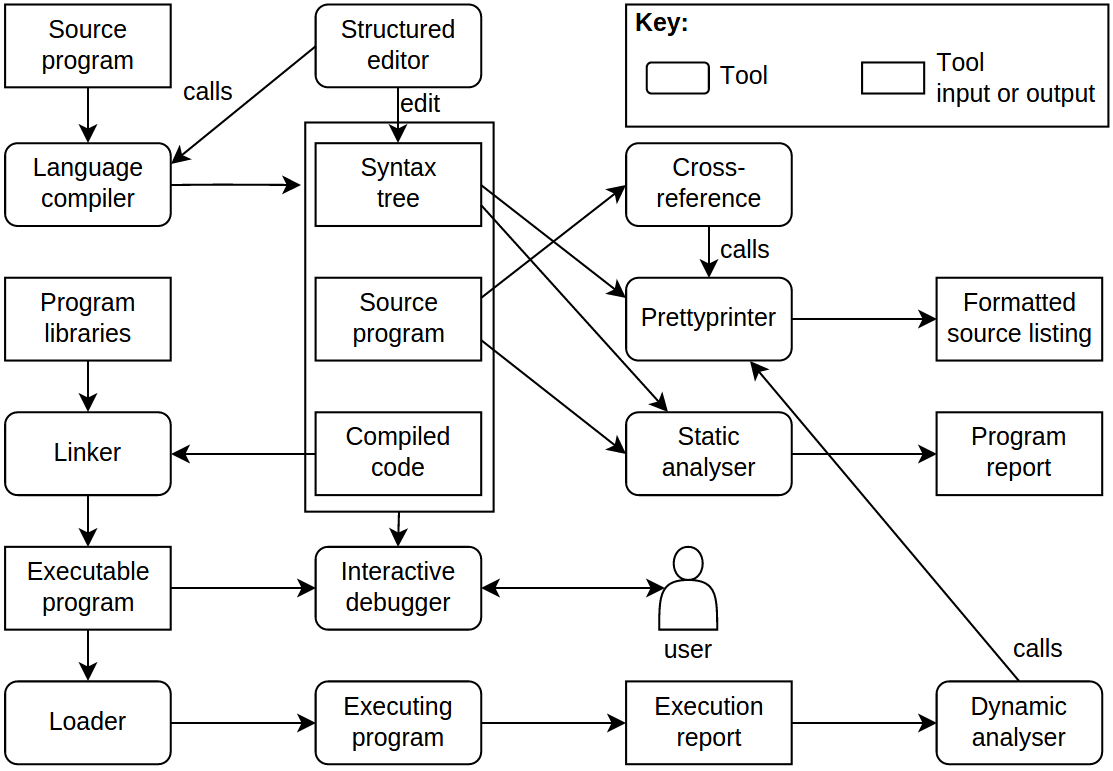
\includegraphics[scale=0.2]{img/pwb}
    \caption{General architecture of a programming environment~\cite{sommerville1996software}. The rounded rectangles represent the tools and the normal rectangles are the tools input or output. The  arrows without label means a tool input (arrow in) or a tool output (arrow out).}
  \label{fig:pwd}
\end{figure}

The central components of this system are assemblers and compilers, which translate higher-level programming languages to machine code. In general, all the data are generated by the compiler, and are used by others components. It is a typical definition of a repository style architecture~\cite[chap.~4.5]{clements2002documenting}, the pool system is the syntactic and semantic information generated from source code during compilation. Mainly, the tools are implement over the artefacts produced by the compiler, as we can see in Figure~\ref{fig:pwd}. So, each tool are described as following:

\begin{itemize}
 \item \textit{Language compiler}. Translates source programs to object node. As part of this translation process, an \ac{ast} and a symbol table is created. Fundamental pieces of future analysis.
 \item \textit{Structured editor}. Incorporates embedded programming language knowledge and edits the syntactic representation of the program in the \ac{ast}, rather than its source code text.
 \item \textit{Linker}. Links the object code program with components which have already been compiled.
 \item \textit{Loader}. Loads the executable program into computer memory prior to execution.
 \item \textit{Cross-referencer}. Produces a cross-reference listing showing where all program names are declared and used.
 \item \textit{Prettyprinter}. Scans the \ac{ast} and prints the source program according to embedded formatting rules.
 \item \textit{Static analyser}. Analyses the source code to discover anomalies such as unitialized variables, unreachable code, uncalled functions and procedures.
 \item \textit{Dynamic analyser}. Produces a source code listing annotated with the number of times each statement was executed when the program was run. It may also generate information on program branches and loops and statics processor usage.
 \item \textit{Interactive debugger}. Allows the user to control the execution sequence and view the program state as execution progress.
\end{itemize}

Among these tools the Interactive debugger in the only one capable to make inferences in a running program. As we show later, it represents the early liveness systems. However, as clever the \ac{ide} does the inference in the \ac{ast} as useful its features will be. In this context, some techniques are used, for example LightTable (describe on Section~\ref{sec:lt}) has to change the Clojure compiler in order to retain more useful meta-data to improve the inference. 

Since to achieve our objective we have to build some tools and integrate them in an existing \ac{ide}, this study have revealed the fundamental pieces of an \ac{ide}. Next, lets turn into the most modern \ac{ide}s in order to understand what features are worth reproducing in a simple and functional \ac{ide} and what features are not.

\subsection{General-purpose IDEs}
\label{sec:ide}

The modern \ac{ide}s, such as Eclipse~\ac{ide}~\cite{carlson2005eclipse}, NetBeans \ac{ide}~\cite{boudreau2002netbeans} and Microsoft Visual Studio~\footnote{\url{http://visualstudio.com}}, support several \ac{pl}s, and also provide a platform for developers to extend their functionalities. For instance, Eclipse provides the called Eclipse Platform~\cite{desrivieres2004eclipse}. Using this platform programmers can write new tools in a form of a plug-in, changing the custom behaviour of the \ac{ide}. For example, the Example Programming Centric~\cite{edwards2004example} is a programming environment with \ac{repl} and interactive tracer on top of Eclipse using the Java \ac{pl}.

Moreover, these \ac{ide}s have many features that work as the programmer writes code, to provide immediate feedback.
So, immediate feedback attempts to show the impact of user's change as soon as possible. For instance, Eclipse~\ac{ide} includes syntax highlighting, code completion suggestions, and indications of problems associated with various locations in source files. Facilities for editing running code also exist. Due to the \ac{jvm} has included a “hot-swap” feature that enables the replacement of a class file by a new one while the overall program is running. That permits \ac{ide}s to offer a code “push” feature to quickly compile a new version of a class and/or object and insert it into the running \ac{jvm}. However, there are more elegant ways to do this, for example using another programming language that fully supports reflection~\cite{bobrow1993clos} mechanisms.

Despite the identified advantages of these \ac{ide}s, they are designed for professional programmers and have a steep learning curve. As concluded in~\cite{Chen:2005:EEI:1089053.1089068}, with experiments using Eclipse, a novice programmer often, does not know the value of an \ac{ide}, therefore ending up avoiding its use. Moreover, it has so many features that overwhelms the learner, and also does not totally support liveness.

\subsection{Liveness in programming environments}
\label{sec:liveness}
The concept of liveness~\cite{tanimoto2013perspective} is an enhancement of the old technique used by the early interactive debuggers. However, liveness \ac{ide}s allow interaction with a running program without stop its execution. In some systems, this is achieved by using a \ac{pl} that supports \textit{reflection}~\cite{bobrow1993clos}, which allows a program to manipulate as data the state of the program during its own execution. On the other hand, is not necessary that a \ac{pl} provide reflection to build a liveness \ac{ide}. Due to \ac{ide}'s architecture (as described on Sec.~\ref{sec:ide}).

In this section, most \ac{ide}s are using a \ac{pl} that supports reflection.

\subsubsection{LightTable IDE}
\label{sec:lt}

\ac{lt}~\cite{lighttable} is an \ac{ide} whose main features are real-time feedback allowing instant execution, debugger with enhanced capabilities to present the program flow and quick access to program documentation. This \ac{ide}, has proved that Victor's ideas~\cite{inventingPrin,learnableProg} were achievable and, indeed, allowed a powerful programming environment. \ac{lt} implemented several of those ideas and serves to us as one example, in order to achieve our objectives.

\ac{lt} was initially written in Clojure~\cite{hickey2008clojure} and actually has moved, almost the full implementation, to ClojureScript. In fact, the success of the \ac{ide}'s features is due to the capabilities of the ClojureScript \ac{pl}. Since, interactive features lacks on a programming model which allows continuous change. As a result, the programming model should manage its state independently of the data, in order that changes in the code does not affect data, such as Smalltalk~\cite{goldberg1983smalltalk} model does. However, in Clojure model code is mostly functional, where continuous code changes can be seen as continuous effects. This language capability allows \ac{lt} to implement gracefully its interactive features over a web based environment.

The Clojure \ac{pl} is a compiled language that compiles the code directly to \ac{jvm} bytecode. In addition, to share with Lisp dialect the code-as-data philosophy, it provides a powerful macro system. In other hand, ClojureScript also has those advantages, however it uses a Clojure compiler which targets JavaScript. As a consequence, it creates powerful features over JavaScript and even remains dynamic. In this way, \ac{lt} represent a web application, which is running inside a little frame running node-webkit~\footnote{\url{https://github.com/rogerwang/node-webkit}} inside it. In reality, it is just {\small HTML}. A easy and quick way to prototype.

Among other features, we will focus on the traceability mechanism and the ability to make the program flow visible. First, the traceability, showed in Figure~\ref{fig:lt1}, and second the real-time debugger in Figure~\ref{fig:lt2}.

The traceability is the ability to relate parts of the program with some additional resources, in order to make the program meaning transparent. In \ac{lt}, a textual mechanism was used to this end. Therefore, when the programmer move the cursor over a function identifier, immediately the available documentation of this function is displayed on a panel, such as in Figure~\ref{fig:lt1}. This feature is useful, because it enables the reader to effortlessly read the program, to decode the code. Then, the programmer can concentrate in what is really genuine.

\begin{figure}[h]
  \centering
  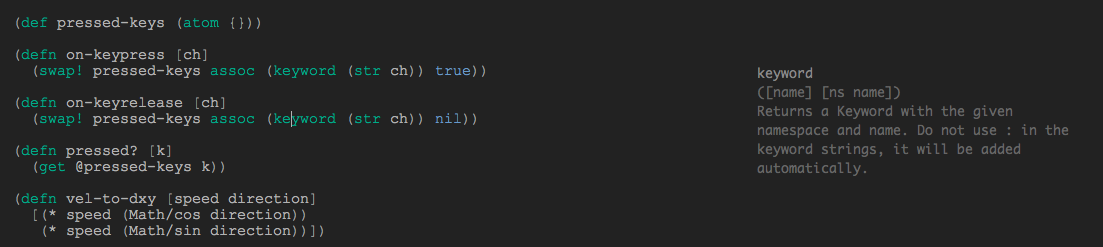
\includegraphics[width=1.0\textwidth]{img/lt2}
    \caption{A program in LightTable \ac{ide}. On the right is the text code editor, the cursor was moved into a function name, i.e. {\tt keyword}. On the left, is a panel where appears the additional documentation of the function, in this case the {\tt keyword} function.}  
  \label{fig:lt1}
\end{figure}

However, it just relates the predefined functions with the existing documentation. The problem to understand the genuine functions yet remains. Moreover, textual resources can be useful in this context, however to other environments is not. For example, in generative design systems, sketches representation, graphics correlation and images are much more explanatory than text representation.  

The reminiscent problem, understand the genuine code, would be mitigated using the real-time debugger. Improving the idea of lispers environment, where we can try out expressions in a \ac{repl}, \ac{lt} goes further by doing it in place, and instantaneously. A common technique of live programming systems~\cite{PER-GRA:2007,sorensen2005impromptu,mclean2010visualisation}. However, \ac{lt} uses reflection mechanisms to show the program flow and its respective values. In Figure~\ref{fig:lt2},  the expression {\tt (x 3 7)} has been evaluated, and the structure of the function {\tt x} was replicated on the panel, however the variables were replaced by their real substitutions.

\begin{figure}[h]
  \centering
  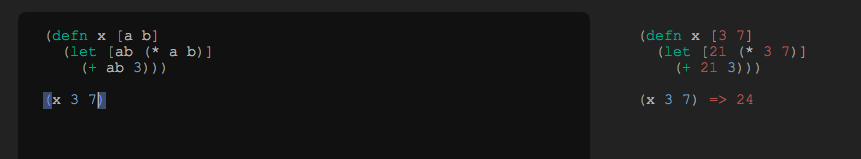
\includegraphics[width=1.0\textwidth,height=0.1\textheight]{img/lt1}
    \caption{A program in LightTable~\ac{ide} being explored using the real-timer debugger feature.}  
  \label{fig:lt2}
\end{figure}

The real-timer debugger allow an interactive way to debug the code and also a meaningful way to understand the program flow. However, for a complex program, seeing the variables replaced by their values will not increase the program meaning, a lot. On the contrary, the programmer will spend as much effort with this feature as without it. Nevertheless, a graphical representation for the program flow seems to be most appropriate. For example, the DrRacket~\ac{ide}~\cite{findler2002drscheme} uses arrows to show the program flow.

Another novel capability of \ac{lt} is dealing with time. As Victor suggests~\cite{learnableProg}, a program can be seen as a game. Thus, the frames are compared to the line-instructions, which is a very fine-grained view of time. As a result, the program should process and handle each frame and its correspondent events, over the program execution. However, old frames, i.e. instructions, can be changed, causing effects in the future execution. For instance, it is a powerful model for game development, since programmers can pause the game adjusting the game's parameters and see the consequence of it, in the future execution. Other system such as PythonTutor~\cite{GuoSIGCSE2013} allow time navigation, through the program execution, using a time travel slider and \ac{lt} provide a stroboscopic visual elements, which projects the future steps of an object. Despite dealing with time be essential in some system, it is not our main concern.

Even though \ac{lt}~\ac{ide} has useful tools for augmenting program comprehension, it was designed for professional programmers. Moreover, the tools are tailored for a general purpose \ac{ide}. However, similar ideas behind these tools has already been implemented by others systems, as we will show next.

\subsubsection{Fluxus}

Fluxus~\footnote{\url{http://www.pawfal.org/fluxus/}} is a live programming environment for 3D graphics, music and games. It  allows, quickly make live animation and audio programs, and change them constantly and flexibly. 

Fluxus supports Racket as \ac{pl}, similar to other live programming systems, such as Impromptu~\cite{sorensen2005impromptu}. Also, the most  interesting feature for us, it supports live programming through the DrRacket~\ac{ide}. Moreover, Fluxus provide a game engine platform which allows, for instance, experiments in visualization of live coding~\cite{mclean2010visualisation}.

%
%\begin{figure}[h]
%  \centering
%  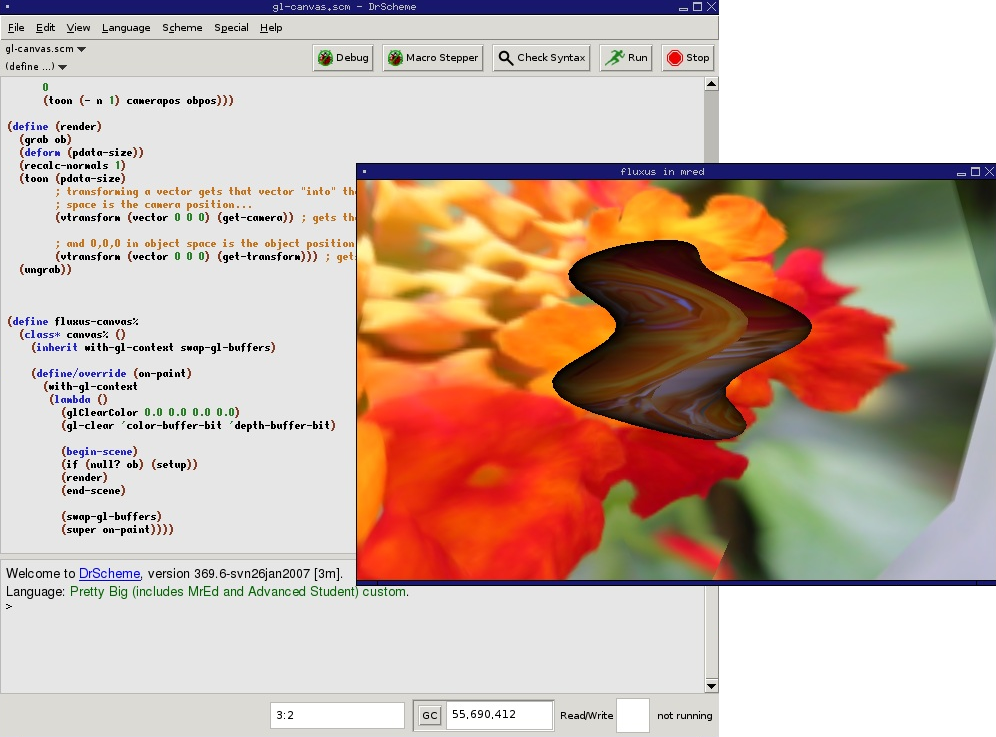
\includegraphics[width=1.0\textwidth]{img/fluxus}
%    \caption{A Fluxus program within DrRacket~\ac{ide}. This program is written in Scheme (as the %Racket was called previously), whose output is a 3D image, on the left.  }
%  \label{fig:fluxus}
%\end{figure}

Although DrRacket~\ac{ide} can be used, Fluxus provides its own programming environment. Including, a text editor which appears in front of the graphics, that the code is generating. In general, this environment works on top of a \ac{repl} with some nuances. The fluxus scripts are not executed directly, it is first written in a text buffer. Just in case it is syntactically correct, it is then interpreted to the target language, in this case {\small C++}. As a result, performers can change the code while the programming still running. Once the program is syntactically correct, the new instructions are immediately executed, consequently changing the graphic window.

In addition, Fluxus does not break the program interactivity, as the program becomes complex. Mainly because, Fluxus uses the OpenGL graphics library, and export several OpenGL functionalities wrapped in the fluxus script. For example, the following instructions will draw a default cube on a OpenGL window. Note that, the instruction at line 6, will be interpreted as a {\small C++} timer callback. In reality, it creates an abstract layer over {\small C++} programming and OpenGL, facilitating the programming and encouraging learning. 

\lstdefinestyle{scheme}{
  language=Lisp,
  basicstyle=\tt\small,
  columns=fullflexible,
  commentstyle=\color{Orange},
  keywordstyle=\color{Blue},
  identifierstyle=\color{Blue},
  stringstyle=\color{Green},
  numbers=left,
  numberstyle=\small\tt,
  frame=lines,
}

\lstset{style=scheme}
\begin{lstlisting}
; start by defining a render function
(define (render)
  (draw-cube)) ; which draws a cube
  
; call render every frame
(every-frame (render))
\end{lstlisting}

However, Fluxus is focused on live artistic performance and its tools reflect this purpose. However, it is a good start point to implement a live environment using the DrRacket~\ac{ide}. 

\subsubsection{IPython}

IPython~\cite{PER-GRA:2007} is an programming environment, developed in a command shell base. Originally, IPython was designed to be a mini Mathematica~\cite{wolfram1991mathematica}, developed in Python~\ac{pl}, once it provides several libraries to math computation. Nowadays, IPython supports a set of languages, i.e. front-ends, and it provides, among other features, an interactive shell with introspection capability, inline data visualization and a browser-based notebook with support for code, text, mathematical expressions, inline plots and other rich media (showed in Figure~\ref{fig:ipython}). 

The main interest in IPython, relies on the fact that it provides a base layer for programming environments. So, IPython exposes its major components to the user for modification and customization. Consequently, would be possible get benefit of IPython features in others systems, once it is an open platform.  

\begin{figure}[h]
  \centering
  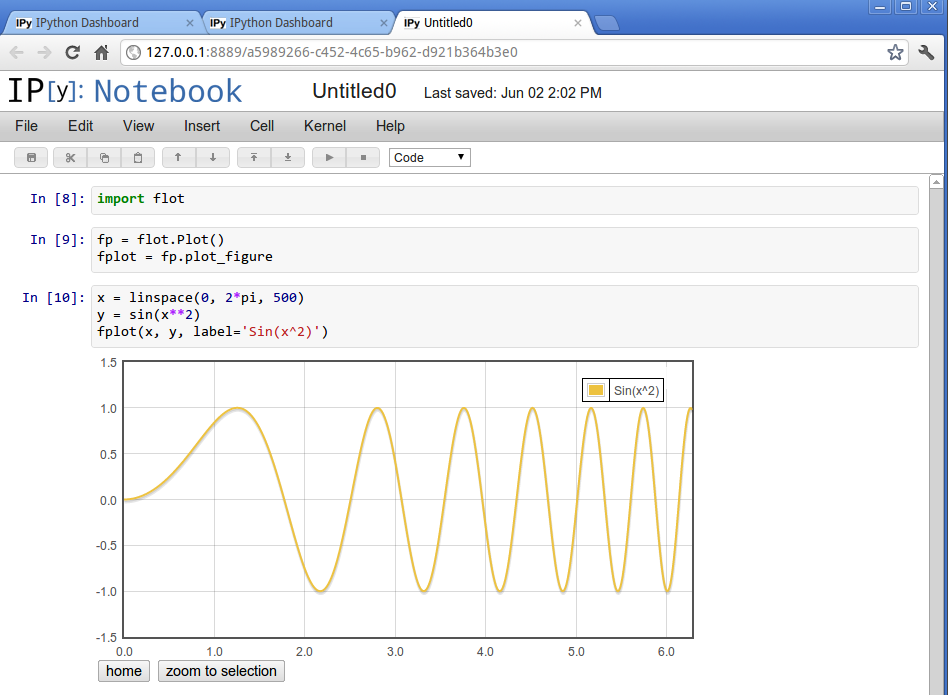
\includegraphics[scale=0.22]{img/ipython}
    \caption{A session interaction using the IPython notebook. Each input is identified with sequence number, e.g. {\tt In[8], ..., In[n]}, which allow to reuse a previous computation result. Also, an input can contain one or more expressions. }  
  \label{fig:ipython}
\end{figure}

The Figure~\ref{fig:ipython}, shows the interactions with IPython notebook. So, IPython architecture is a type of client-server, where the front-end is the client, in this case a notebook, and the server is a language kernel. The language kernel is a \ac{pl} which the user interacts. As a result, this mechanism gives IPython a certain level of interoperability, in order to support new \ac{pl}s. However, a strict communication protocol must be implemented by the kernel. On the other hand, the communication is very robust using the ZeroMQ~\cite{hintjens2013zeromq} networking and concurrency library. Certainly, it is a good example in order to support interactive tools in a real system environment.

Actually, the DrRacket~\ac{repl} has similar functionality of a command shell. In sense that, the expressions typed in the \ac{repl} are immediately evaluated and its result displayed. However, it does not support plots nor rich media visualisation. On the other hand, some experiments in adapting the DrRacket~\ac{repl} to support 3D graphics visualisation has revealed interesting results, is the case of Pitct3D~\footnote{\url{https://github.com/ntoronto/pict3d}} a successful integration of DrRacket~\ac{repl} within OpenGL.

A inherent concern behind a live programming model is the security. Since in a live programming environment, in principle, the instructions are executed immediately, there must exist some mechanism that guarantees the permissiveness of the code being executed. In order to understand how it could be done, lets see the next system. 

\subsubsection{PythonTutor}

PythonTutor~\cite{GuoSIGCSE2013} is a web-base live coding environment that allows Python learns to write the code and navigate step by step throughout the programming structures. PythonTutor is a pedagogical system and, as well as \ac{lt}, it splits the program execution in steps, allowing the learners to navigate through the steps. However, our concern is on the security mechanism implemented, since in our system security is a concern.

The situation becomes worse in PythonTutor, because it has a server (back-end) which takes the untrusted Python code from the web, and execute it. In order to prevent the execution of dangerous constructs such as {\tt eval}, {\tt exec} and {\tt file I/O},  PythonTutor implements sandboxing. Basically, it denies the use of most module imports, by parsing the user's code importing. A strict approach, but effective.

\subsection{Programming environment for GD}
\label{sec:gd}

This section presents the area of generative design, as well as the existing systems and its limitations. A study was devised to analyse the programming environments that supports \ac{vpls}, and \ac{tpls}.

\subsubsection{The generative design}

In the area of architecture, \ac{gd} is a design method that uses an algorithm to generate an architectural model~\cite{terzidis2003expressive}. As a consequence of the \ac{gd} integration into the design process, the development of novel design solutions, difficult or even impossible to achieve via other methods~\cite{mccormack2004generative}, is now possible. However, this method supposes: (1) the use of a programming language, in order to specify the algorithm and (2) a programming environment with, at least, a language interpreter or compiler and a source code editor, to assist this process.

The use of \ac{gd} methods has become popular, mainly between designers and architects. Increasingly, many people without any background in Computer Science has written simple scripts and, indeed, have appeared new script languages and new environments to this end. For example, from \ac{vpls} environments such as Grasshopper and Dynamo to \ac{tpls} environments such as  VisualLisp, Processing, RhinoScript and Rosetta. Next we describe each one.

\subsubsection{Visual programming environments}
In this context, the visual programming environment are those which support the \ac{vpls}. The \ac{vpls} can be seen as a bi-dimensional representation consisting of iconic components that can be interactively manipulated by the user according to some spatial grammar~\cite{myers1990taxonomies}. In general, the components are represented as boxes, meaning shapes or operations over shapes. The boxes can be connected to others boxes, also known as components. It establishes a dataflow between components, such that the output of a component is the input of another. For example, the Figure~\ref{fig:grass} represent a program in Grasshopper that computes the coordinates of a conical spiral, and Figure~\ref{fig:dynamo} represent a program in Dynamo.


\begin{figure}[h]
  \centering
  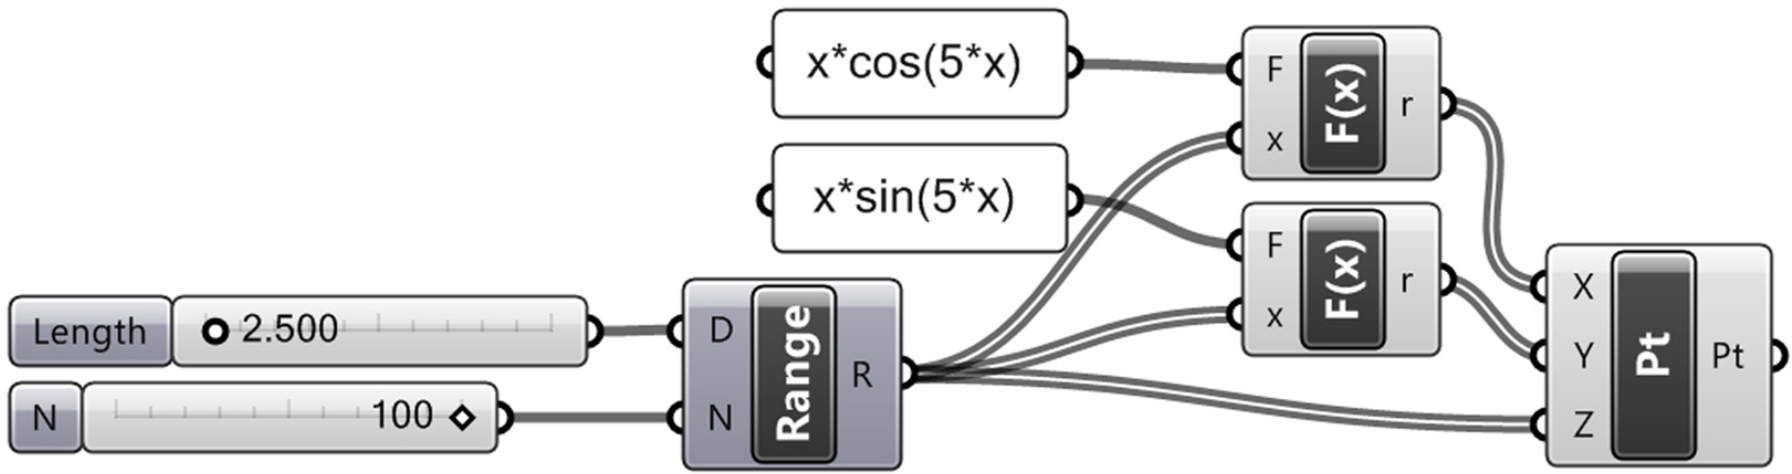
\includegraphics[scale=0.15]{img/grasshopper}
    \caption{A program in Grasshopper that computes the 3D coordinates of a conical spiral. On the left, two sliders connected to the program input. A change in the slider recomputes the new coordinate.}
  \label{fig:grass}
\end{figure}

Grasshopper is one the most popular environments for \ac{vpls}, as a result, it will be used as the programming environment representative of \ac{vpls}. It is implemented as a plug-in over Rhinoceros3D~\footnote{\url{https://www.rhino3d.com}}. However, it provides its own \ac{ide}, which is very attractive for the designers community, mainly for those beginners in \ac{gd}. Due to the fact of Grasshopper provides features of an environment dedicated for learning. As an example of these features are: 

\begin{itemize}
 \item Immediate feedback. As the user interacts with the components, by adding and connecting them, the result of this interaction is immediately visible, on the geometric model in Rhino.  It is because, Grasshopper is constantly updating the Rhino's model, upon the user's change. Consequently, it facilitates the design conception, since the user's intentions are immediately visible. So, users has no more the boring task to compile-run the program, also can endeavour in design exploration.
 \item Input widget. To facilitate the process of design exploration, Grasshopper provides sliders which are connected at the program's input. So, as the users dragged the sliders, the program are recomputed, with the slider's value. As result, new models are generated and can be visualised. A easy way to test new set of values, as well as augmenting the program comprehension.
 \item Traceability. As another form of feedback, occurs when the designer selects a component, and then, the geometry generated by that component is highlighted, in the model. Consequently, the designers can quickly understand the program, by figuring out the roles of each component.
 \item Show comparisons. By adding a new component in an existing program it is possible to replicate all the geometry generated by that program. As a result, an old geometry is maintained in background while a new one is changed. Thus, the designer can compare the result of his change in the new geometry based on the old one. This technique is very useful, because adds a context at each change. So, it is easier understanding data by comparing it to other data.
\end{itemize}

However, these tools suffers on limitations. For instance, immediate feedback is suitable for small programs, where the model is regenerated in real-time. So, for large and complex programs, the time needed to propagate the values through all the program components is unreasonable. As a result, the interactivity is broken and this feature will be avoided. Also, the traceability will be even more useful, whether it supports the reverse association. Finally, for the comparisons be showed, the designer should add another component to the program. It requires that he understands the program, or at least the main data flow, in order to use this feature. Unlike this approach, this feature should be available whenever a change in the model occurs.

Another popular environment for \ac{vpls} is the Dynamo~\footnote{\url{http://dynamobim.com/}}. However, Dynamo is implemented on top of Revit, a specifically software for \ac{bim}. In despite of being similar to the Grasshopper features, there are features in Dynamo which are worth seeing. First, is the ability to add watchers to the output nodes. In Figure~\ref{fig:dynamo}, a single point is being showed in three views, (1) textually in the watch, (2) graphically in the watch 3D and (3) in the model, at background. It allows inspect individually each node, a good form for augmenting the program comprehension, and also, to find bugs. However, that implies adding more nodes into the program and figuring out where is the best place to add them. Second, it has a lateral table which provides more than simply quick access. It also, encourages the designers to explore the available nodes and try new nodes never ever tried. A powerful feature to get new ideas. 

\begin{figure}[h]
  \centering
  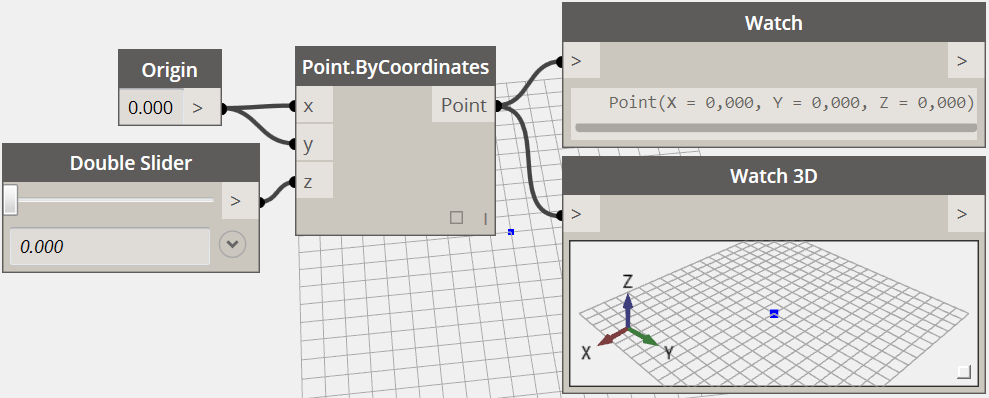
\includegraphics[scale=0.3]{img/dynamo}
    \caption{A program in Dynamo which calculates a single 3D point. The x and y coordinate are fixed at origin and, the z coordinate varies as the slider are dragged. On the right, two representations of watch. Note that, the background of the image, also is showing the point.}
  \label{fig:dynamo}
\end{figure}

The programming environments that supports \ac{vpls} are popular between the novice programmers. The smooth learn curve, and perhaps the style of the \ac{ui} elements, are attractive for beginners. However, as the {\small VPL} programs become large and complex it requires more time to understand, maintain, and adapt to new requirements, than {\small TPL} programs~\cite{leitao2011programming}. So, despite spending more time and effort to learn \ac{tpls}, the learners have their time quickly recovered, once the complexity of the design task becomes sufficiently large. For this, lets see the available programming environments for \ac{tpls}.

\subsubsection{Textual programming environments}

In general, the programming environment for \ac{gd}, usually contains a language editor, a language interpreter or a compiler and just few provides a debugger. 

Initially, AutoCAD provides the VisualLisp environment which has, a text editor, an interpreter and a debugger. The main problem with this environment, was not the environment itself, but was in the supported programming language, AutoLisp. So, AutoLisp is a very old dialect of Lisp, obsolete and has several problems~\cite{cabecinhas2010high}. Similarly happens with the \ac{vba} for AutoCAD and its \ac{pl} Visual Basic (a descendant of {\small BASIC}). Recently, the Autodesk's DesignScript~\cite{aish2012designscript} overcomes several of those \ac{pl} problems. 

The DesignScript's programming environment provides a text editor coupled into the AutoCAD, an interpreter and a debugger. For instance, the debugger can be used as an interactive feature. In Figure~\ref{fig:ds}, in each step of the debugger, a variable is set. According to the associative paradigm of the \ac{pl}, changing this value causes a change-propagation. In other words, whenever this variable occurs it will reflect its new value. As a result, a new model is recomputed and displayed. So, this environment works in a kind of live programming.

\begin{figure}[h]
  \centering
  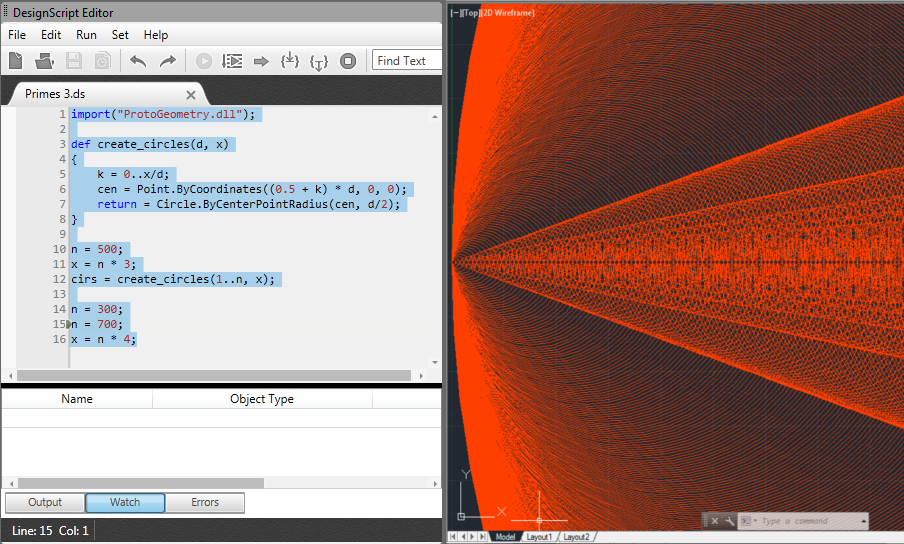
\includegraphics[scale=0.25]{img/designScript}
    \caption{A DesignScript program, on the left, whose output represents graphically the sieve of Eratosthenes, on the right. This ancient algorithm for finding all prime numbers, is being tested interactively using the DesignScript's debug feature. }
  \label{fig:ds}
\end{figure}

Although DesignScript's environment provide live programming, it does not support several useful features which helps in design conception. For example: 

\begin{itemize}
 
\item The DesignScript language, does not fully supports sliders, so common in live programming environment. However, the integration with the \ac{ide} does. But, the changes in the sliders are not immediately seen in the model, just when the slider is dropped. In this situation, the designer should imagine what would be the value dragged, completely against the purpose of the sliders. 

\item Also, there is a fragile mechanism of traceability. First, it is necessary to add a watch in a variable then inspect its result in the watch tab (see Figure~\ref{fig:ds}). If the contents of a variable represent a geometric model then the respective model is highlighted. However the inverse traceability is not supported. 

\item In addition, the text editor just supports a linear sequence of characters. So, is not possible to illustrate the code, with design sketches. 

\item Finally, a drastic problem, the performance. A common problem with \ac{cad} application renders due to slow operation processing. So, the \ac{cad}s are not prepared for the huge volume of operations generated by the \ac{gd} methods. As result, the interactivity of the live programming feature will only lead to small and simple programs. Some effort in the direction of sidestepping this problem, is being taken by replace the \ac{cad} render by a faster render, for instance using OpenGL graphics library. 
\end{itemize}

Similarly to the embedded DesignScript editor, the current Monkey editor for Rhino4~\footnote{\url{http://wiki.mcneel.com/developer/monkeyforrhino4}} can be used to edit, run, debug and compile scripts. It performs automatic syntax parsing by colouring and indenting keywords, auto-completion and error highlighting. Also, it provides a multi-document interface, code trees and integrated help files. However, it does not support none of the previous features described and also it was not an environment thought to be pedagogical.

On the other hand, Processing~\footnote{\url{https://processing.org/}} a \ac{pl} and \ac{ide}~(Fig.~\ref{fig:pross}), developed by the {\small MIT} media,  was created to teach programming to students, artists, and designers, without any previous programming experience~\cite{reas2006processing}. In order to do this, Processing uses a visual context, using
a software sketchbook of 2D and 3D designs implemented on top of an OpenGL renderer. In addition, it provides different programming modes that enable the user to create new sketches in different languages and platforms.

\begin{figure}[h]
  \centering
  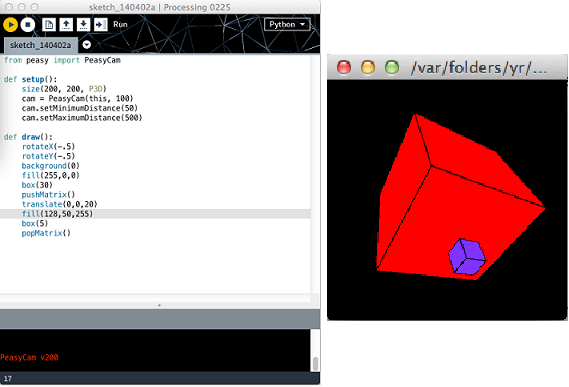
\includegraphics[scale=0.4]{img/processing}
    \caption{On the left, a processing program whose output, on the right, represents two cubes. The program was written in Python an its output was rendered in a OpenGL window.}
  \label{fig:pross}
\end{figure}

By using the Processing~\ac{ide} designers can have a quick overview of their designs (an example of a Processing design is presented in Fig.~\ref{fig:pross}). Moreover, it has good documentation which is supported by a large open-source community and by a significant academic critical mass. However, for a more complex modelling tasks Processing fails to offer a viable solution. Although Processing allows to create models in several \ac{pl}s, its \ac{ide} just uses the OpenGL render.   

Rosetta~\cite{lopes2011portable}, by contrast, allows the interoperability between different \ac{cad} applications with different \ac{pl}s. 

Usually, designers used to be locked-in to one family of \ac{cad} application, when developing their projects. Consequently, their designs were totally system-dependent, e.g. just work on specific \ac{cad}, and platform-dependent, e.g. just work in a certain operative system. Obviously, it creates strict requirements that hinders the design conception. In order to overcome this problem, Rosetta suggested a portable \ac{gd} for \ac{cad}~\cite{lopes2011portable}. It allows the use of different \ac{pl}s (front-ends) and interoperates with different \ac{cad} applications (back-ends). For example in Figure~\ref{fig:rosetta1}, Rosetta is being used with front-end Racket and back-end AutoCAD. The execution of the \ac{gd} program, produces the following geometric model.

\begin{figure}[h]
  \centering
  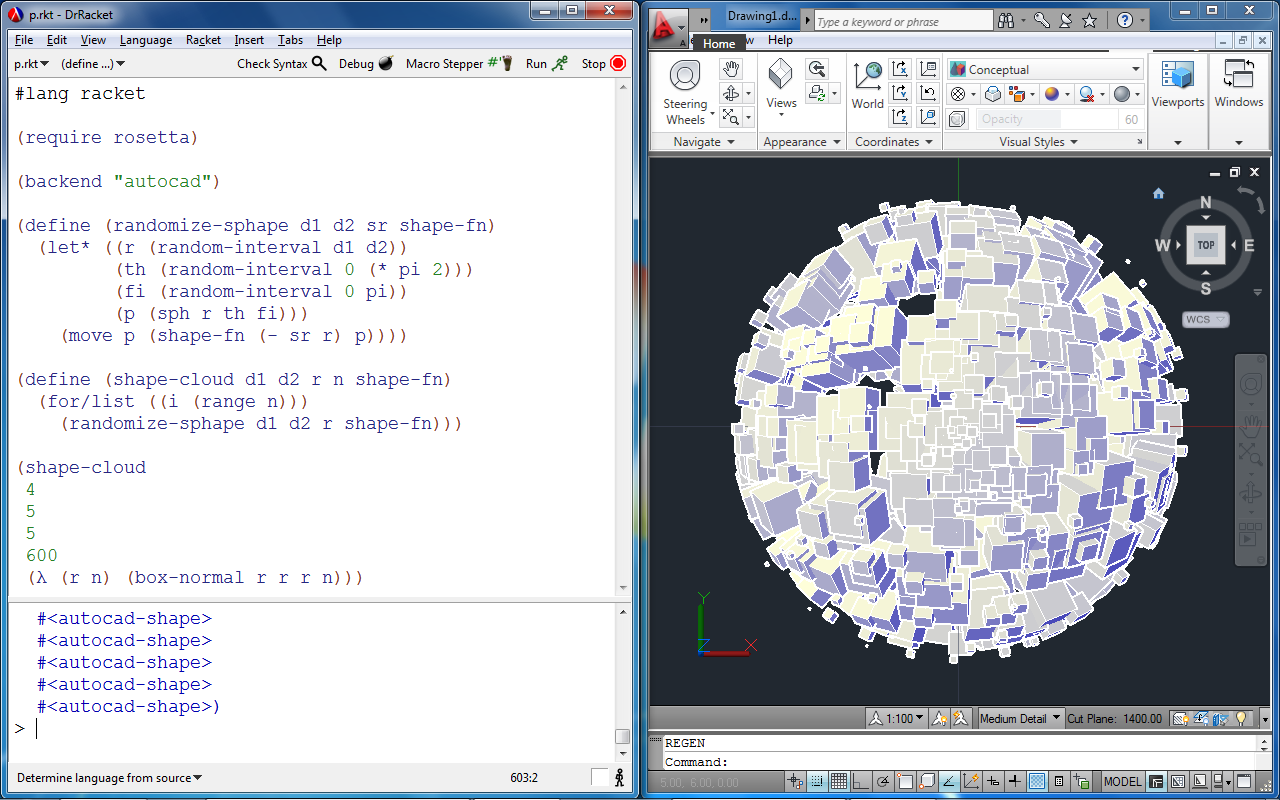
\includegraphics[scale=0.2]{img/rosetta1}
    \caption{A Rosetta program, on the left, and its output, on the right. The program was written in Racket using the DrRacket~\ac{ide} and its output was rendered by AutoCAD.}  
  \label{fig:rosetta1}
\end{figure} 

Actually, the front-end is composed by several \ac{pl}s, such as Scheme, AutoLisp, JavaScript, Racket, Python and RosettaFlow (a graphical language inspired in Grasshopper). Moreover, the supported back-ends are the \ac{cad} applications, AutoCAD and Rhinoceros3D. Also, there have been experimental alternative back-ends, e.g. based on OpenGL, in response to performance needs. As the project is being developed, new front-ends are going to be created, such as Processing. Also new back-ends, such as Revit, MicroStation and ArchiCAD.

By following this approach, the generated design left to be a merely \ac{cad} application (strictly system-dependent) and pass to be implemented by an algorithm. As a result, the design can be reproduced by several \ac{cad}s, even in others platforms~\cite{lopes2011portable}.

Despite the identified advantages, there are, at least, three important drawbacks associated with the Rosetta's programming environment. Although DrRacket~\ac{ide} (a descendant of DrScheme~\cite{findler2002drscheme}) be considered as pedagogical~\cite{findler2002drscheme}, we can point out the problems as follows:

\begin{itemize}
 \item \textit{Poor or non-existent context explanation.} A program in Rosetta is an algorithm description of a geometric design. However, there is none correlation shown between the intend design, the \ac{gd} program and its generated model. Thereby, in order to understand a \ac{gd} program, designers must find by themselves this correlation, spending a significant mental effort, unnecessarily. 
 
 \item \textit{Users cannot see the program flow.} To produce a geometric model, the computer traces a path through the code, looping around loops and calling into several functions and incrementally building up the output. We see none of this. As a result, designers should imagine what the program is doing, again an avoidable mental effort.
 
 \item \textit{Do not provide immediate feedback.} Most part of designers' work is an attempt to create art. That means, for instance, try over and over new parameters for parametric functions never ever found. Actually, that is a laborious and tedious process, hence in each attempt the program must be executed manually.
\end{itemize}





